%%%%%%%%%%%%%%%%%%%%%%%%%%%%%%%%%%%%%%%%%%%%%%%%%%%%%%%%%%%%%%%%%%%%%%%%%%%%%%%%%%
\begin{frame}[fragile]\frametitle{}
\begin{center}
{\Large Implementation}
\end{center}
\end{frame}


%%%%%%%%%%%%%%%%%%%%%%%%%%%%%%%%%%%%%%%%%%%%%%%%%%%%%%%%%%%
\begin{frame}[fragile]\frametitle{}

\begin{center}
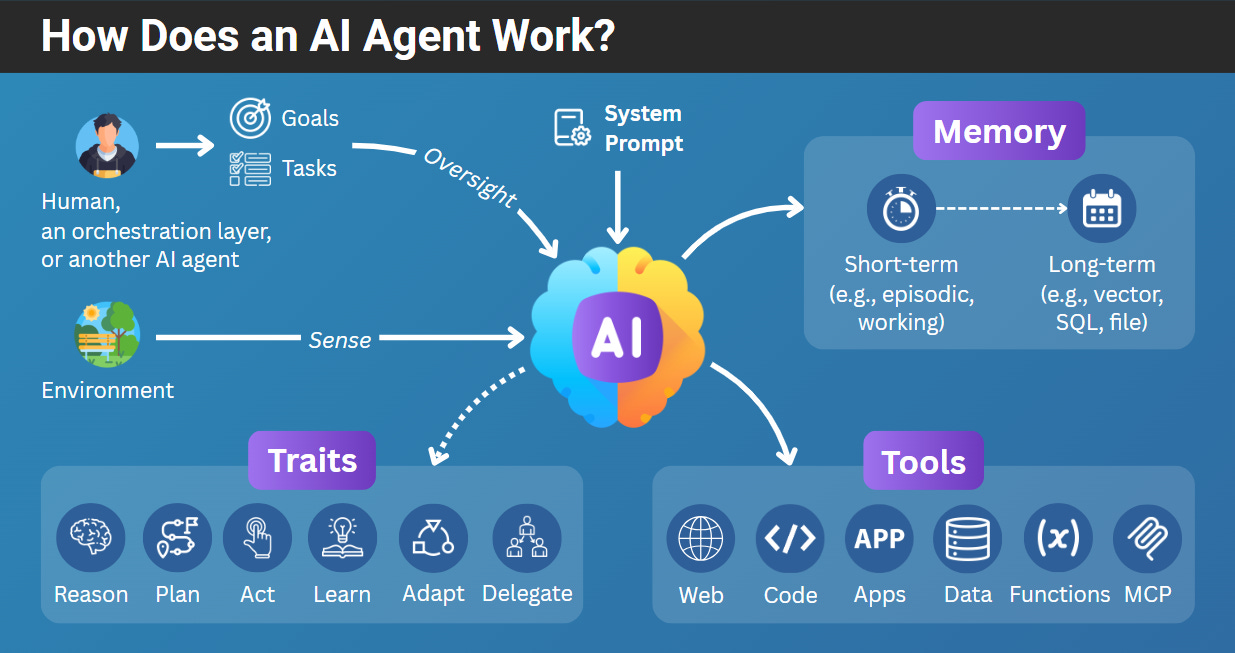
\includegraphics[width=\linewidth,keepaspectratio]{aiagents5}

{\tiny (Ref: The Ultimate Guide to AI Agents for PMs - Pawl Huryn)}
\end{center}	
  
\end{frame}

%%%%%%%%%%%%%%%%%%%%%%%%%%%%%%%%%%%%%%%%%%%%%%%%%%%%%%%%%%%
\begin{frame}[fragile]\frametitle{Build Your First AI Agent}
      \begin{itemize}
        \item Takes just 30-60 minutes to get started
        \item Follow a clear step-by-step process
        \item Focus on functionality, not theory
      \end{itemize}
\end{frame}

%%%%%%%%%%%%%%%%%%%%%%%%%%%%%%%%%%%%%%%%%%%%%%%%%%%%%%%%%%%%%%%%%%%%%%%%%%%%%%%%%%
\begin{frame}[fragile]\frametitle{How to Build an AI Agent?}

	\begin{center}
	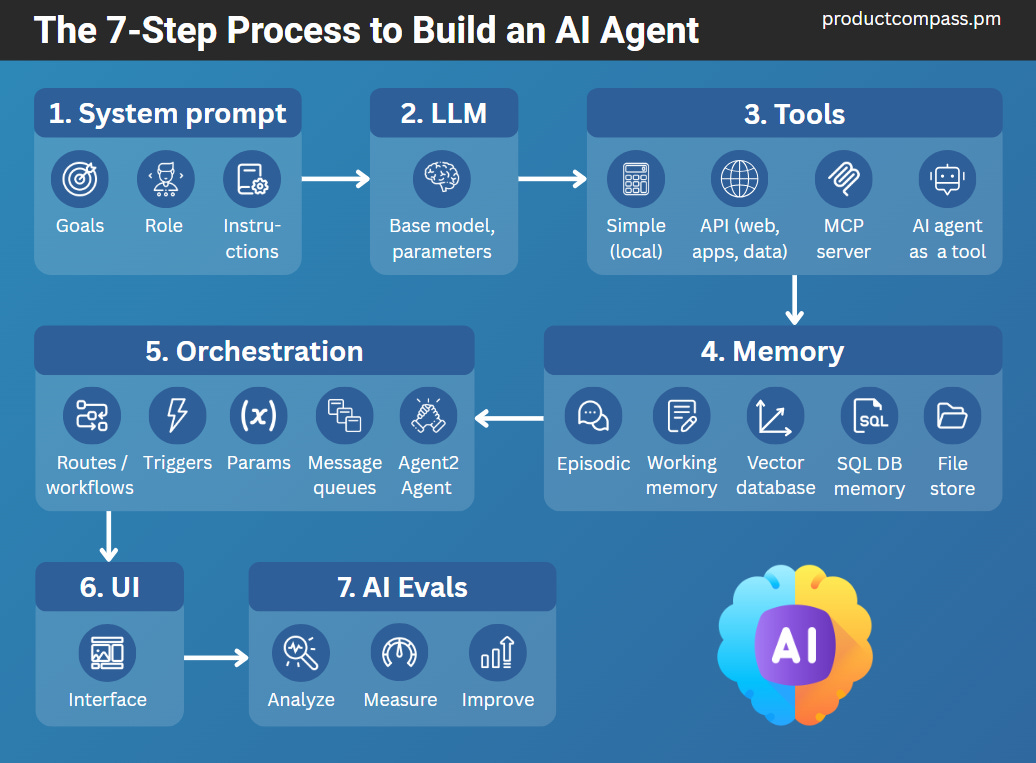
\includegraphics[width=0.8\linewidth,keepaspectratio]{aiagents7}
	\end{center}
	
	{\tiny (Ref: The Ultimate Guide to AI Agents for PMs - Pawl Huryn)}
\end{frame}


%%%%%%%%%%%%%%%%%%%%%%%%%%%%%%%%%%%%%%%%%%%%%%%%%%%%%%%%%%%
\begin{frame}[fragile]\frametitle{Step 1: Define a System Prompt}
      \begin{itemize}
        \item Set goals, logic, and expectations
        \item Use structured prompting principles
        \item Refer to expert guides for inspiration
      \end{itemize}
\end{frame}

%%%%%%%%%%%%%%%%%%%%%%%%%%%%%%%%%%%%%%%%%%%%%%%%%%%%%%%%%%%
\begin{frame}[fragile]\frametitle{Step 2: Select an LLM}
      \begin{itemize}
        \item Choose a reasoning-capable model (e.g., o1-mini)
        \item Frameworks like n8n may handle iterations
        \item Pick based on your use case complexity
      \end{itemize}
\end{frame}

%%%%%%%%%%%%%%%%%%%%%%%%%%%%%%%%%%%%%%%%%%%%%%%%%%%%%%%%%%%
\begin{frame}[fragile]\frametitle{Step 3: Connect Tools}
      \begin{itemize}
        \item Add tools based on agent goals
        \item Use calculators, functions, data sources
        \item Optional: MCP servers for integration
      \end{itemize}
\end{frame}

%%%%%%%%%%%%%%%%%%%%%%%%%%%%%%%%%%%%%%%%%%%%%%%%%%%%%%%%%%%
\begin{frame}[fragile]\frametitle{Step 4: Connect Memory}
      \begin{itemize}
        \item Enable short-term memory for local state
        \item Use long-term memory: vector, SQL, graph
        \item Essential for tracking progress and context
      \end{itemize}
\end{frame}

%%%%%%%%%%%%%%%%%%%%%%%%%%%%%%%%%%%%%%%%%%%%%%%%%%%%%%%%%%%
\begin{frame}[fragile]\frametitle{Step 5: Orchestrate the Logic}
      \begin{itemize}
        \item Map core logic not tied to a single agent
        \item Enable agent-to-agent communication
        \item Static or dynamic flows via orchestration
      \end{itemize}
\end{frame}

%%%%%%%%%%%%%%%%%%%%%%%%%%%%%%%%%%%%%%%%%%%%%%%%%%%%%%%%%%%
\begin{frame}[fragile]\frametitle{Step 6: Add User Interface}
      \begin{itemize}
        \item Use no-code tools like Lovable or Bolt
        \item Easily create interfaces without coding
        \item Great for user-facing agents and SaaS apps
      \end{itemize}
\end{frame}

%%%%%%%%%%%%%%%%%%%%%%%%%%%%%%%%%%%%%%%%%%%%%%%%%%%%%%%%%%%
\begin{frame}[fragile]\frametitle{Step 7: Evaluate the Agent}
      \begin{itemize}
        \item Skip fixed metrics-do error analysis
        \item Let performance metrics emerge naturally
        \item For RAG: evaluate retrieval and generation separately
      \end{itemize}
\end{frame}

%%%%%%%%%%%%%%%%%%%%%%%%%%%%%%%%%%%%%%%%%%%%%%%%%%%%%%%%%%%
\begin{frame}[fragile]\frametitle{Bottom Line: Just Start}
      \begin{itemize}
        \item Follow practical guides-many require no coding
        \item Use frameworks like n8n and tools like MCP
        \item Stop theorizing-start shipping real systems
      \end{itemize}
\end{frame}


%%%%%%%%%%%%%%%%%%%%%%%%%%%%%%%%%%%%%%%%%%%%%%%%%%%%%%%%%%%%%%%%%%%%%%%%%%%%%%%%%%
\begin{frame}[fragile]\frametitle{}
\begin{center}
{\Large Practical Tips}
\end{center}
\end{frame}

%%%%%%%%%%%%%%%%%%%%%%%%%%%%%%%%%%%%%%%%%%%%%%%%%%%%%%%%%%%
\begin{frame}[fragile]\frametitle{RAG vs. Fine-Tuning: Business Impact}
    \begin{itemize}
        \item Business-critical systems require the right LLM strategy.
        \item Fine-tuning feels powerful, but often adds avoidable complexity.
        \item Start by exploring simpler and more flexible approaches first.
    \end{itemize}
\end{frame}

%%%%%%%%%%%%%%%%%%%%%%%%%%%%%%%%%%%%%%%%%%%%%%%%%%%%%%%%%%%
\begin{frame}[fragile]\frametitle{RAG vs SFT}
	
	\begin{center}
	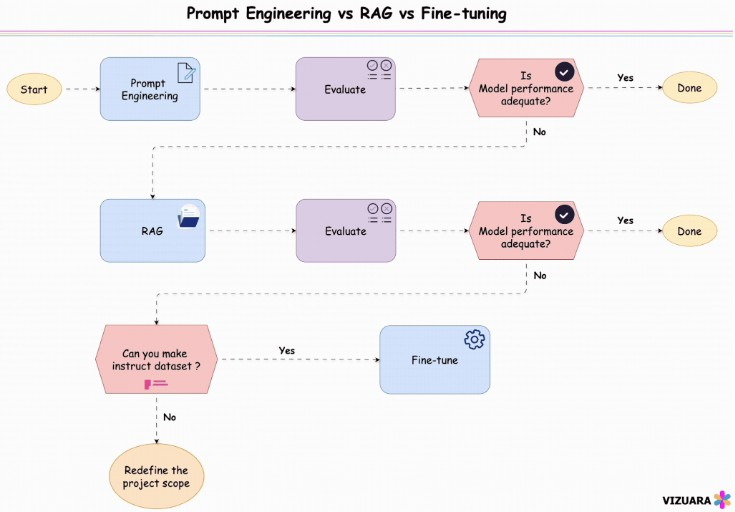
\includegraphics[width=0.8\linewidth,keepaspectratio]{vizuara1}
	\end{center}
	
{\tiny (Ref: LinkedIn post by Raj Dandekar)}

\end{frame}


%%%%%%%%%%%%%%%%%%%%%%%%%%%%%%%%%%%%%%%%%%%%%%%%%%%%%%%%%%%
\begin{frame}[fragile]\frametitle{Pre-Fine-Tuning Checklist}
    \begin{itemize}
        \item Can prompt engineering alone solve the task?
        \item Could Retrieval-Augmented Generation (RAG) help more?
        \item Is there a clear and testable system already in place?
    \end{itemize}
\end{frame}

%%%%%%%%%%%%%%%%%%%%%%%%%%%%%%%%%%%%%%%%%%%%%%%%%%%%%%%%%%%
\begin{frame}[fragile]\frametitle{Why RAG Outperformed Fine-Tuning}
    \begin{itemize}
        \item \textbf{Higher Accuracy}: Grounded answers from relevant context.
        \item \textbf{Fewer Hallucinations}: More reliable than fine-tuned outputs.
        \item \textbf{Dynamic Updates}: Easily update data without retraining models.
    \end{itemize}
\end{frame}

%%%%%%%%%%%%%%%%%%%%%%%%%%%%%%%%%%%%%%%%%%%%%%%%%%%%%%%%%%%
\begin{frame}[fragile]\frametitle{When to Use Fine-Tuning}
    \begin{itemize}
        \item RAG can't solve context window limitations.
        \item Domain-specific tone or behavior is required.
        \item The system is mature enough to absorb added complexity.
    \end{itemize}
\end{frame}

%%%%%%%%%%%%%%%%%%%%%%%%%%%%%%%%%%%%%%%%%%%%%%%%%%%%%%%%%%%
\begin{frame}[fragile]\frametitle{Strategy Summary}
    \begin{itemize}
        \item Prompt engineering solves 30--50\% of tasks.
        \item RAG adds power for another 30--40\%.
        \item Fine-tuning is best for the final 10\% of hard problems.
        \item Always choose the simplest effective approach first.
    \end{itemize}
\end{frame}

%%%%%%%%%%%%%%%%%%%%%%%%%%%%%%%%%%%%%%%%%%%%%%%%%%%%%%%%%%%
\begin{frame}[fragile]\frametitle{A2A MCP ADK}
	
	\begin{center}
	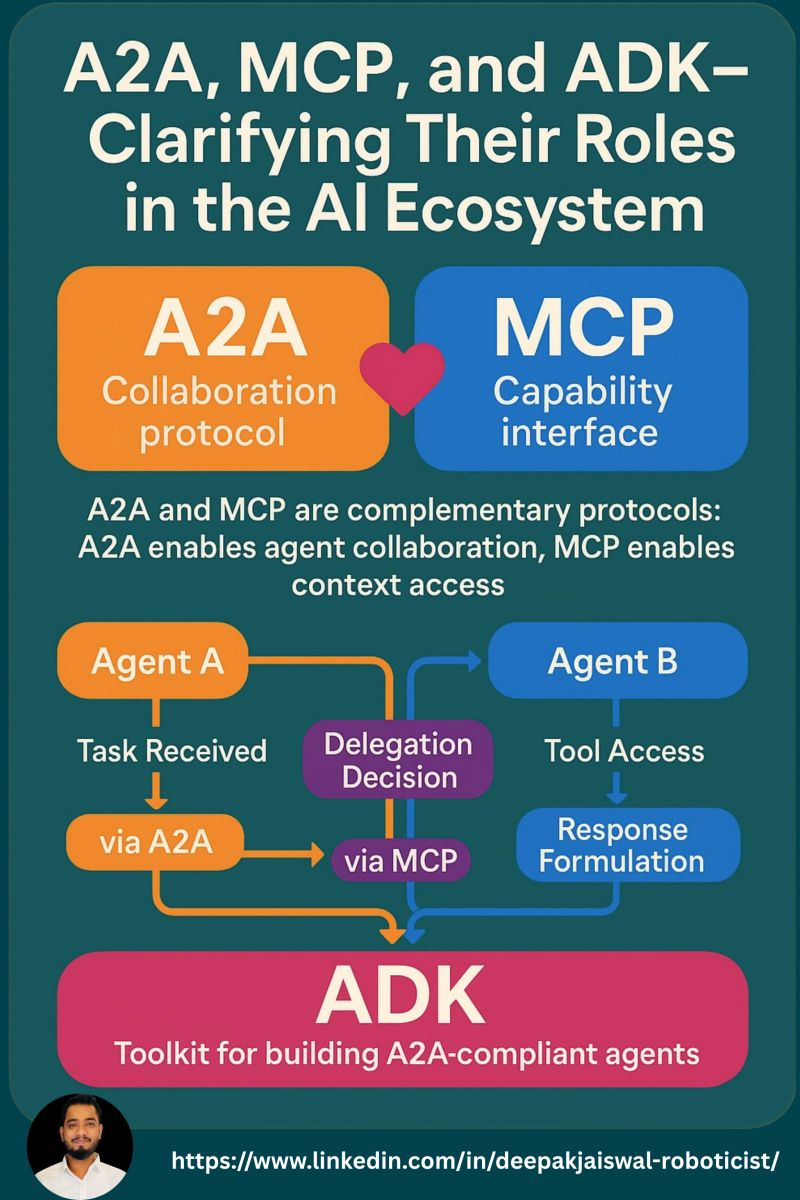
\includegraphics[width=0.4\linewidth,keepaspectratio]{agents7}
	\end{center}
	
{\tiny (Ref: LinkedIn post by Deepak Jaiswal)}

\end{frame}

%%%%%%%%%%%%%%%%%%%%%%%%%%%%%%%%%%%%%%%%%%%%%%%%%%%%%%%%%%%
\begin{frame}[fragile]\frametitle{Agentic AI Protocols Overview}
    \begin{itemize}
        \item A2A, MCP, and ADK are foundational for agentic systems.
        \item Each solves a unique challenge in building autonomous agents.
        \item They work together to enable scalable multi-agent architectures.
    \end{itemize}
\end{frame}

%%%%%%%%%%%%%%%%%%%%%%%%%%%%%%%%%%%%%%%%%%%%%%%%%%%%%%%%%%%
\begin{frame}[fragile]\frametitle{A2A: Agent-to-Agent Protocol}
    \begin{itemize}
        \item Enables agent discovery, delegation, and communication.
        \item Facilitates coordination in distributed multi-agent systems.
        \item Example: Agent A delegates a task to Agent B and receives results.
    \end{itemize}
\end{frame}

%%%%%%%%%%%%%%%%%%%%%%%%%%%%%%%%%%%%%%%%%%%%%%%%%%%%%%%%%%%
\begin{frame}[fragile]\frametitle{MCP: Model Context Protocol}
    \begin{itemize}
        \item Standardizes agent access to tools, APIs, and data.
        \item Ensures consistent, secure interaction with external systems.
        \item Example: Agent queries a database or triggers a payment via MCP.
    \end{itemize}
\end{frame}

%%%%%%%%%%%%%%%%%%%%%%%%%%%%%%%%%%%%%%%%%%%%%%%%%%%%%%%%%%%
\begin{frame}[fragile]\frametitle{ADK: Agent Development Kit}
    \begin{itemize}
        \item Toolkit for building A2A-compliant agents quickly.
        \item Includes libraries and scaffolds for rapid development.
        \item Compatible with frameworks like CrewAI, LangGraph, Semantic Kernel.
    \end{itemize}
\end{frame}

%%%%%%%%%%%%%%%%%%%%%%%%%%%%%%%%%%%%%%%%%%%%%%%%%%%%%%%%%%%
\begin{frame}[fragile]\frametitle{How They Work Together}
    \begin{itemize}
        \item \textbf{MCP}: Makes agents powerful with tool access.
        \item \textbf{A2A}: Enables inter-agent collaboration.
        \item \textbf{ADK}: Simplifies and accelerates agent development.
    \end{itemize}
\end{frame}

%%%%%%%%%%%%%%%%%%%%%%%%%%%%%%%%%%%%%%%%%%%%%%%%%%%%%%%%%%%
\begin{frame}[fragile]\frametitle{Real-World Analogy}
    \begin{itemize}
        \item \textbf{MCP}: Tools in a mechanic's toolbox.
        \item \textbf{A2A}: Team communication and task-sharing.
        \item \textbf{ADK}: Blueprint for building each mechanic fast.
    \end{itemize}
\end{frame}

%%%%%%%%%%%%%%%%%%%%%%%%%%%%%%%%%%%%%%%%%%%%%%%%%%%%%%%%%%%
\begin{frame}[fragile]\frametitle{Why This Stack Matters}
    \begin{itemize}
        \item Forms the backbone of enterprise AI, robotics, and automation.
        \item Enables modular, scalable, and intelligent agentic systems.
        \item Quickly becoming a standard for future AI workflows.
    \end{itemize}
\end{frame}
